\documentclass[tikz,border=4pt]{standalone}
\usepackage{amsmath}
\begin{document}
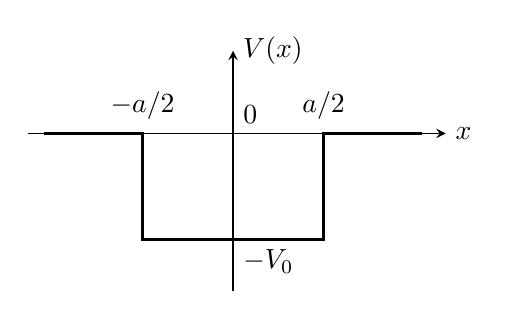
\begin{tikzpicture}[>=stealth, thick, scale=1.0]
  % Axes
  \draw[->, line width=0.5pt] (-2.6, 0) -- (2.7, 0) node[right] {$x$};
  \draw[->, line width=0.5pt] (0, -2.0) -- (0, 1.05) node[right] {$V(x)$};
  \node[above right] at (0, 0) {$0$};

  % Potential well: width a (-a/2 to a/2), depth -V0
  \draw[line width=1.1pt] (-2.4, 0) -- (-1.15, 0) -- (-1.15, -1.35) -- (1.15, -1.35) -- (1.15, 0) -- (2.4, 0);

  % Labels
  \node[above] at (-1.15, 0.05) {$-a/2$};
  \node[above] at (1.15, 0.05) {$a/2$};
  \node[below right] at (0, -1.35) {$-V_0$};
\end{tikzpicture}
\end{document}
